% !TeX spellcheck = si_SI
\chapter{Pregled rešitev}\label{cha:metodologija}

Kot smo spoznali v prejšnjem poglavju, uporaba zemljevidov z visko ločljivostjo ni upravičena, saj je poraba računalniških sredstev tako prevelika. Naša naloga je najti način glajenja grobe poti, osnovane na zemljevidu z nizko ločljivostjo in rešitev implementirati. V kontekstu ROS-a bo potrebno ustvariti vmesno vozlišče, ki bo prestreglo sporočila grobe poti, jih transformirala v gladko pot ter posredovla avtonomnemu vozilu. Pri implemetaciji je zaželena tudi enostavnost in intuitivnost implemetacije rešitve skozi oči uporabnika.

\section{Pregled možnih rešitev}

Navdih za rešitev problema glajenja poti smo dobili na področju motornih športov. Tam se vozniki dirkalnih vozil izključno poslužujejo načina vožnje skozi ovinke, ki rezultira v tako imenovani dirkalni liniji (ang. \textit{Racing Line}). Dirkalna linija je pot preko ovinka, ki vozniku dirkalnika omogoča najkrajši čas proge \cite{vir2}. Želja je, da je hitrost pri vožnji skozi ovinek kar se da konstantna.

\begin{figure}[H]
	\centering
	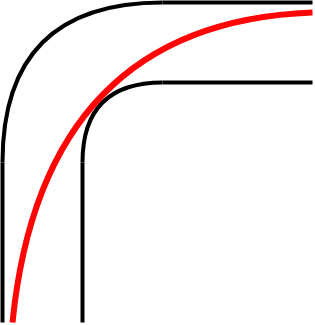
\includegraphics[width=3cm]{pic/slika4.png}
	\caption{Dirkalna linija.}
	\label{fig:slika}
\end{figure}

Ideja za dirkalno linijo je ta, da se vozilo oklepa zunanjega roba ovinka pri vstopu v ovinek in se skuša kar se da približati notranjemu robu ovinka na njegovem vrhu. Na izhodu iz ovinka pa se vozilo ponovno približa zunanjemu robu. V teoriji je optimalna pot skozi ovinek takšna, ki ima največji radij.

Iskanje najboljše dirkalne linije za dano vozilo, na dani progi je eden od večjih problemov s katerim se srečujejo razvijalci dirkalnih računalniških iger \cite{vir3}. Komercialne dirkalne igre se ponavadi zanašajo na dirkalne linije, ki jih zasnujejo ljudje - strokovnjaki s področja dirkanja. Obstajajo pa tudi izjeme, ki se izognejo omenjeni metodi in se problema lotijo na povsem drugačen način. Dober primer je Colin McRae Rally, kjer dirkalno linijo računajo s pomočjo nevronske mreže, ki so jo učili strokovnjaki iz področja motornih športov \cite{vir3}. V Microsoft-ovi igri Forza Motorsport 2 s pomočjo tehnik nadzorovanega učenja (ang. \textit{Supervised Learning}) učijo AI-je ter z aplikacijo evolucijskega računanja (ang. \textit{Evolutionary Computation}) optimirajo njihove dirkalne linije \cite{vir4}.

Odprtokodne dirkalne igre se ponavadi zanašajo na hevristične pristope, ki tipično združujejo dobro prakso s hevristiko pri generaciji dirkalnih linij. Najuspešnejši primeri takšnih pristopov vključujejo K1999 algoritem \cite{vir5}, ki ga je razvil Remi Coulom in deluje na podlagi gradientnega spusta (ang. \textit{Gradient Descent}) ter Simplix \cite{vir6}, ki ga je razvil Wolf-Dieter Beelitz za The Open Car Racing Simulator in bazira na preprosti hevristiki. Ostala uspešna primera sta tudi \textit{the bot} \cite{vir7}, ki ga je razvil Jussi Pajala za Robot Auto Racing Simulator (RARS) in je zasnovan na A* algoritmu ter the \textit{DougE1 bot} za RARS, ki ga je razvil Doug Elenveld, ta pa izkorišča genetski algoritem. Kljub temu, da omenjene rešitve temeljijo na različnih tehnikah je vsem skupno to, da skušajo zmanjšati ukrivlejnost poti vozila skozi ovinek, saj z manjšo ukrivlejnostjo poti vozilo lahko doseže večjo hitrost brez zdrsa.

Zgoraj omenjene metode so sicer zelo impresivne, vendar obstajajo tudi metode, ki upoštevajo dinamski model vozila pri reševanju omenjenega problema in vodijo do še ustreznejših rešitev omenjenega problema. Na drugi strani pa imamo rešitve, ki so malce preprostejše kot je uporaba kubičnih parametričnih Bézier krivulj pri generaciji dirkalne linije \cite{vir8} in pa edinstvena rešitev, ki jo nudi odprtokodni Vamos Avtomotive Simulator, kjer je za doesganje manjše ukrivlejnosti poti skozi ovinek uporabljena vergia masnih točk, ki jih povezuje torzijska vzmet. Do gladke poti pridemo tako, da iščemo minimum potencialne energije shranjene v vzmeteh. Pri reševanju našega problema smo se odločili za seldnjo metodo, zato jo bomo v naslednjem podpoglavju predstavili podrobneje.

\section{Izbrana rešitev}

Vamos Avtomotive Simulator (VAS) je odprtokodno simulacijsko okolje s poudarkom na fizičnemu modeliranju \cite{vir9}. Vamos modelira veliko večino ključnih podsistemov avtomobilov, kot so elementi pogonskega sklopa in sicer motor, sklopka, menjalnik in diferencial z omejenim zdrsom. Prav tako pa je modelirano tudi obnašanje pnevmatik pri temperaturnih vplivih, vzmetenje avtomobila in aerodinamski učinki na avtomobilih. VAS igralcem nudi tudi igranje proti računalniškemu nasprotniku. V ta namen so razvijalci ustvarili algoritem izgradnje poti za računalniškega nasprotnika tako, da igralcem nudijo karseda realističen izziv. Ta algoritem bomo v naslednjem delu besedila vzeli pod drobnogled in ga nato tudi uporabili pri reševanju našega problema.

\subsection{VAS algoritem}

Pot vozila na začetku predstavlja nabor točk, ki tvorijo središčnico znotraj proge. Točke predstavimo kot masne točke, ki so med seboj povezane s torzijskimi vzmetmi.

\begin{figure}[H]
	\centering
	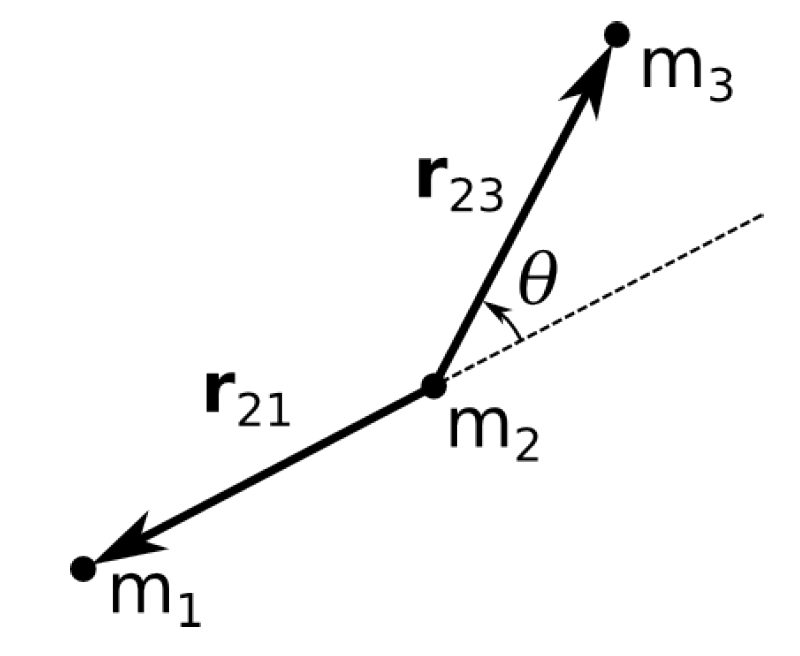
\includegraphics[width=4cm]{pic/slika5.png}
	\caption{Tri vozlišča poti. Moment pri kotu $\theta$ \cite{vir9}.}
	\label{fig:slika}
\end{figure}

Tak sistem bo s časom silil v stanje minimalne energije v torzijskih vzmeteh in nam posledično ustvaril pot z manjšo ukrivljenostjo.

Silo, ki deluje na maso $m_2$ je možno izračunati na podlagi relativnih leg sosednjih mas. Začnimo s sklepom, da s povečanjem kota $\theta$ dobimo moment sorazmeren kotu.
\begin{equation}
\mathbf{N_2} = \mathbf{r}_{23} \times \mathbf{F_3} = -k \theta \hat{n}
\end{equation}
Pri tem je $\mathbf{r}_{23}$ vektor od $m_2$ do $m_3$ in $\hat{n}$ je enotski vektor, ki kaže v smeri $\mathbf{r}_{23} \times \mathbf{r}_{21}$. Sila na $m_3$ je tako:
\begin{equation}
\mathbf{F_3} = -\frac{k}{|\mathbf{r}_{23}|}\theta(\hat{n} \times \mathbf{r}_{23})
\end{equation}
Produkt $\theta \hat{n}$ se izračuna kot vektorski produkt $\mathbf{r}_{23}$ in $\mathbf{r}_{21}$.
\begin{equation}
\mathbf{r}_{23} \times \mathbf{r}_{21} = |\mathbf{r}_{23}||\mathbf{r}_{21}| \sin(\phi - \theta) \hat{n}
\end{equation}
\begin{equation}
\sin\theta\hat{n} = |\mathbf{r}_{23}||\mathbf{r}_{21}|\sin\theta\hat{n}
\end{equation}
\begin{equation}
\sin\theta\hat{n} = \frac{\mathbf{r}_{23} \times \mathbf{r}_{21}}{|\mathbf{r}_{23}||\mathbf{r}_{21}|}
\end{equation}
\begin{equation} \label{eq:1}
\sin\theta\hat{n} = \hat{r}_{23} \times \hat{r}_{21}
\end{equation}
Ker pričakujemo majhne kote med vozlišči lahko $\sin\theta$ zapišemo kot $\theta$.
\begin{equation} \label{eq:2}
\theta\hat{n} = \hat{r}_{23} \times \hat{r}_{21}
\end{equation}
Z vstavljanjem v enačbo $(2)$ dobimo:
\begin{equation}
\mathbf{F}_3 = \frac{k}{|\mathbf{r}_{23}|}(\hat{r}_{23} \times \hat{r}_{21}) \times \hat{r}_{23}
\end{equation}
Upoštevajoč simetrijo ugotovimo, da je $\mathbf{F}_1 = \mathbf{F}_3$ in $\mathbf{F}_2 = -2\mathbf{F}_3$ pri majhnem kotu. Definiramo lahko vektor urkivljenosti $\mathbf{c}$ pri $m_3$:
\begin{equation}
\mathbf{c} = \hat{n}/R = \theta \hat{n} / |\mathbf{r}_{23}|
\end{equation}
Kjer je $R$ radij ukrivljenosti. Kot $\theta$ je kot med $m_2$ in $m_3$ od centra ukrivljenosti.

Enačbo lahko zapišemo kot:
\begin{equation}
\mathbf{F}_3 = -k \mathbf{c} \times \hat{r}_{23}
\end{equation}
Velikost vekotrja ukrivljenosti bomo uporabili kot največjo hitrost vozila v dani točki na stezi.

Sile so izračunane za vsak povezan trojček n točk. Pri tem omejimo gibanje točk v vse smeri in namesto tega dovolimo le pomik prečno na pot. Ta omejitev nam omogoča večjo stabilnost, posledično pa lahko uporabljamo večje togostne koeficiente vzmeti in tako dobimo hitrejšo konvergenco.

Ko je izračunana skupna sila na vsakemu vozlišču lahko izračunamo novo lego točke z uporabo Newtonov-ovih zakonov gibanja ter z Euler-jevo metodo.

\begin{equation}
F = m \ddot{x} + c \dot{x}
\end{equation}

\begin{equation}
\ddot{x} = \frac{F}{m} - \frac{c}{m} \dot{x}
\end{equation}

Kvocient koeficienta dušenja in mase označimo z $d = c / m$.

\begin{equation}
\frac{\dot{x}_{i+1} - \dot{x}_i}{\Delta t} = \frac{F}{m} - d \dot{x}_i
\end{equation}

\begin{equation}
\dot{x}_{i+1} = \dot{x}_i + (\frac{F}{m} - d \dot{x}_i)\Delta t
\end{equation}

Iz definicije hitrosti sledi še druga enačba.

\begin{equation}
\dot{x} = \frac{x_{i+1} - x_i}{\Delta t}
\end{equation}

\begin{equation} \label{eq:16}
x_{i + 1} = x_{i} + \dot{x}_{i + 1} \Delta t 
\end{equation}

Tako dobimo enačbo s katero lahko iterativno določimo novo lego vsake točke poti, ki jo gladimo. Algoritem vsebuje dva paramtera in sicer maso $m$ in kvocient $d$. Pri tem se je potrebno zavedati, da je nova pot lahko groba v ostrih ovinkih (Enačba \ref{eq:1} in \ref{eq:2}).

Spodnje slike prikazujejo delovanje dejanskega algoritma glajenja. Leva slika prikazuje graf niza točk nad katerimi bomo  izvajali glajenje. Sredinska slika prikazuje pravokotne poti po katerih bodo točke spreminjale svoj položaj z iteriranjem algoritma. Te pravokotne poti posameznih točk tvorijo tudi progo. Proga je ključna za glajenje poti, saj določa območje v katerem ga izvajamo. Na desni sliki vidimo niz točk v novi legi.

\begin{figure}[H]
	\centering
	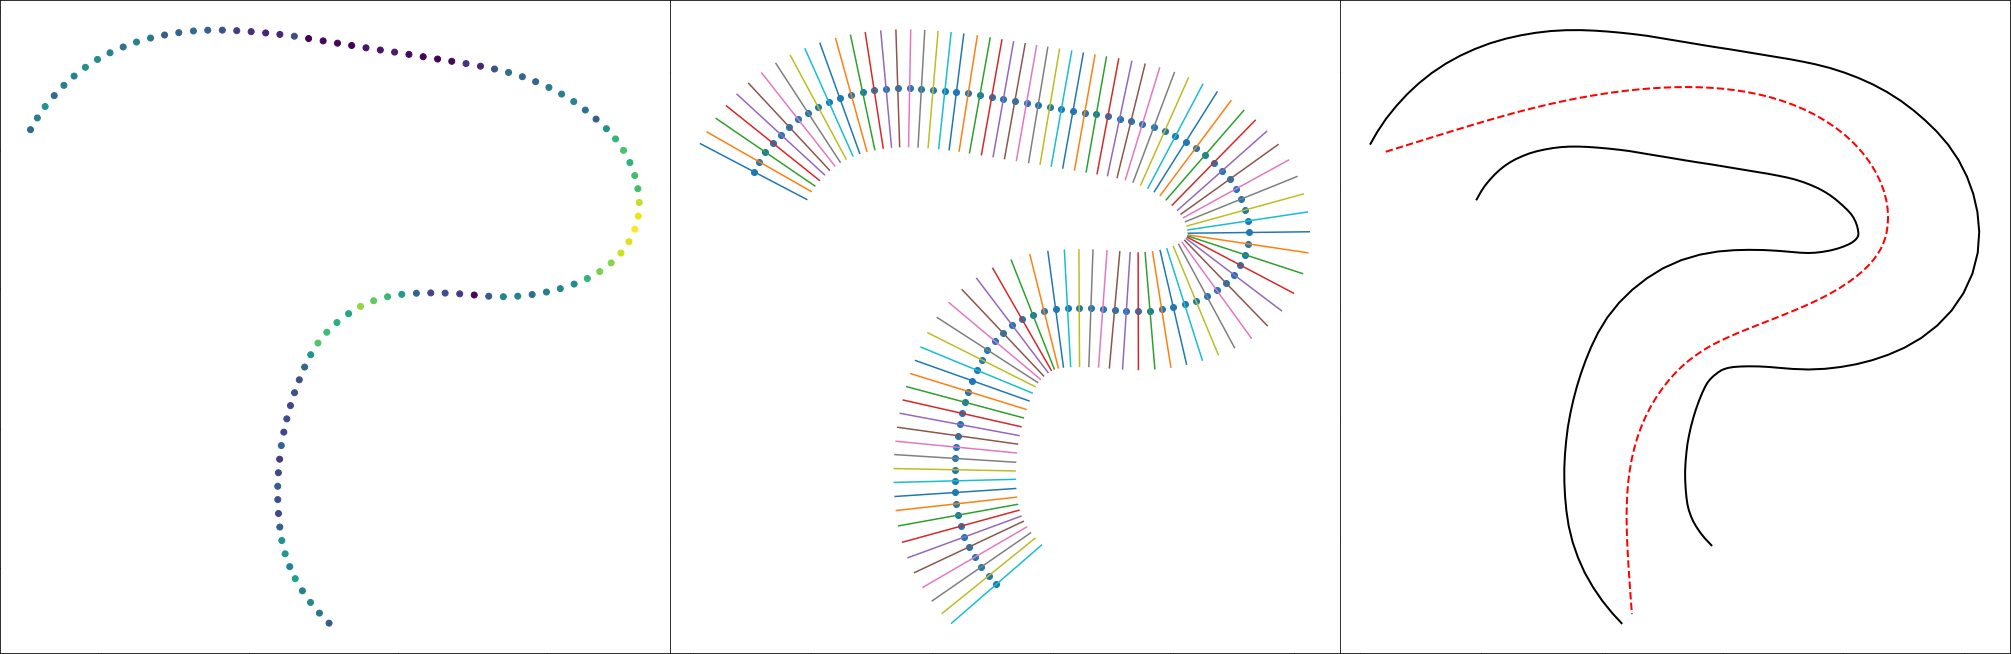
\includegraphics[width=15cm]{pic/slika6.png}
	\caption{Postopek glajenja.}
	\label{fig:slika}
\end{figure}


%V tem poglavju glede na tip naloge (raziskovalni ali razvojni) predstavite, razložite in utemeljite uporabljene \textbf{metode oz. postopke} meritev, izračunov, modelirnih postopkov itn. ter predstavite in utemeljite izbor uporabljenih \textbf{materialov in vzorcev}. V tem poglavju posebej razdelajte tudi merilno negotovost.
%
%\section{Preračuni}\label{sec:preracuni}
%
%Na podlagi predpostavk o \ldots smo za preračun \ldots uporabili izpeljavo \ldots Lorem ipsum dolor sit amet, consectetur adipiscing elit, sed do eiusmod tempor incididunt ut labore et dolore magna aliqua. Ut enim ad minim veniam, quis nostrud exercitation ullamco laboris nisi ut aliquip ex ea commodo consequat. Duis aute irure dolor in reprehenderit in voluptate velit esse cillum dolore eu fugiat nulla pariatur. Excepteur sint occaecat cupidatat non proident, sunt in culpa qui officia deserunt mollit anim id est laborum. 
%
%\section{Eksperimentalni del}\label{sec:eksperiment}
%\subsection{Vzorci in materiali}\label{sec:vzorci}
%\subsubsection{Zobniški par}\label{sec:zobniski_par}
%Za zobniški par smo izbrali \ldots Lorem ipsum dolor sit amet, consectetur adipiscing elit, sed do eiusmod tempor incididunt ut labore et dolore magna aliqua. Ut enim ad minim veniam, quis nostrud exercitation ullamco laboris nisi ut aliquip ex ea commodo consequat. Duis aute irure dolor in reprehenderit in voluptate velit esse cillum dolore eu fugiat nulla pariatur. Excepteur sint occaecat cupidatat non proident, sunt in culpa qui officia deserunt mollit anim id est laborum.
%
%\subsubsection{Gred}\label{sec:gred}
%Gred je bila izdelana iz \ldots Lorem ipsum dolor sit amet, consectetur adipiscing elit, sed do eiusmod tempor incididunt ut labore et dolore magna aliqua. Ut enim ad minim veniam, quis nostrud exercitation ullamco laboris nisi ut aliquip ex ea commodo consequat.
%
%
%\subsection{Metodologija preizkusov}\label{sec:metodologija}
%\subsubsection{Zobniško preizkuševališče}\label{sec:zobn_experiment}
%Zasnovali smo \ldots Lorem ipsum dolor sit amet, consectetur adipiscing elit, sed do eiusmod tempor incididunt ut labore et dolore magna aliqua. Ut enim ad minim veniam, quis nostrud exercitation ullamco laboris nisi ut aliquip ex ea commodo consequat. Duis aute irure dolor in reprehenderit in voluptate velit esse cillum dolore eu fugiat nulla pariatur. Excepteur sint occaecat cupidatat non proident, sunt in culpa qui officia deserunt mollit anim id est laborum.
%
%Lorem ipsum dolor sit amet, consectetur adipiscing elit, sed do eiusmod tempor incididunt ut labore et dolore magna aliqua. Ut enim ad minim veniam, quis nostrud exercitation ullamco laboris nisi ut aliquip ex ea commodo consequat. Duis aute irure dolor in reprehenderit in voluptate velit esse cillum dolore eu fugiat nulla pariatur. Excepteur sint occaecat cupidatat non proident, sunt in culpa qui officia deserunt mollit anim id est laborum.
%
%\subsubsection{Merilnik pomikov (LVDT)}\label{sec:LVDT}
%Za merjenje \ldots smo uporabili linearno variabilni diferencialni transformator (LVDT), s čimer smo zagotovili \ldots Lorem ipsum dolor sit amet, consectetur adipiscing elit, sed do eiusmod tempor incididunt ut labore et dolore magna aliqua. Ut enim ad minim veniam, quis nostrud exercitation ullamco laboris nisi ut aliquip ex ea commodo consequat. Duis aute irure dolor in reprehenderit in voluptate velit esse cillum dolore eu fugiat nulla pariatur. Excepteur sint occaecat cupidatat non proident, sunt in culpa qui officia deserunt mollit anim id est laborum.
%
%\subsection{Analiza deformacijskih mehanizmov}\label{sec:def_mehanizmi}
%Po preizkusih smo površine analizirali z \ldots Lorem ipsum dolor sit amet, consectetur adipiscing elit, sed do eiusmod tempor incididunt ut labore et dolore magna aliqua. Ut enim ad minim veniam, quis nostrud exercitation ullamco laboris nisi ut aliquip ex ea commodo consequat.
%
%\section{Korelacija preračunov in eksperimentalnih rezultatov}\label{sec:korelacija}
%Lorem ipsum dolor sit amet, consectetur adipiscing elit, sed do eiusmod tempor incididunt ut labore et dolore magna aliqua. Ut enim ad minim veniam, quis nostrud exercitation ullamco laboris nisi ut aliquip ex ea commodo consequat. Duis aute irure dolor in reprehenderit in voluptate velit esse cillum dolore eu fugiat nulla pariatur. Excepteur sint occaecat cupidatat non proident, sunt in culpa qui officia deserunt mollit anim id est laborum.
%
%Lorem ipsum dolor sit amet, consectetur adipiscing elit, sed do eiusmod tempor incididunt ut labore et dolore magna aliqua. Ut enim ad minim veniam, quis nostrud exercitation ullamco laboris nisi ut aliquip ex ea commodo consequat. Duis aute irure dolor in reprehenderit in voluptate velit esse cillum dolore eu fugiat nulla pariatur. Excepteur sint occaecat cupidatat non proident, sunt in culpa qui officia deserunt mollit anim id est laborum.


